\chapter{Preparation}

\section{Theory}

\subsection{Slab Waveguide}
\subsubsection{Calculation of Modes}
\subsubsection{Field Distribution and Dispersion Diagramm}


\subsection{Strip Waveguide}



\section{Questions}

\subsection{Slab and Strip waveguide?}
\label{q1}

\subsection{Different performance between TE and TM @ boundary}

\subsection{Single Mode strip waveguide}

\begin{figure}%
\centering
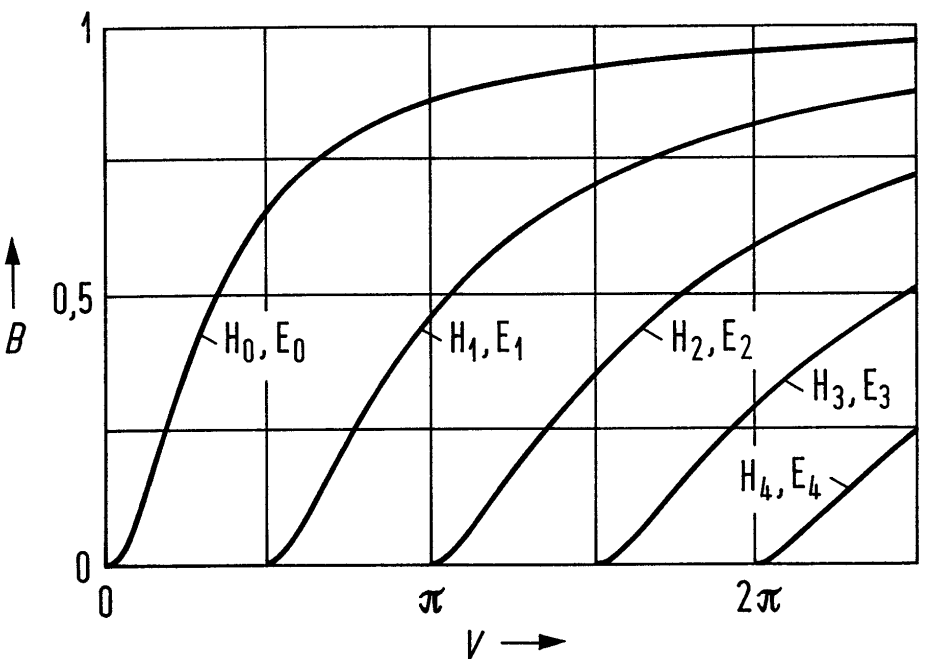
\includegraphics[width=.5\columnwidth]{Grafiken/SingleMode.png}%
\caption{Normalized propagation $B$ over normalized frequency $V$.}%
\label{fig:singlemoded}%
\end{figure}
To achieve a single mode strip waveguide the normalized frequency $V$ needs to be smaller than $V=\pi/2$. As in Figure \ref{fig:singlemoded}\footnote[1]{Wolfgang Freude, Optische Wellenleiter und Sender, Lecture Notes} shown for $V < \pi/2$ only the fundamental mode can propagate. There are still two polarizations H$_0$ and E$_0$.

Using \begin{equation}
V=ak_0\sqrt{n_1^2-n_2^2}
\label{eq:norm_freq}
\end{equation}
with $2a$ is the thickness of the core, $n_1$ is the refractive index of the core, $n_2$ is the refractive index of the surrounding material and $k_0$ is the wavenumber, the the requirements to the waveguide design can be derived.
For the in \ref{q1} assumed values for $n_1$ and $n_2$ this leads to a core-thickness of
\begin{equation}
2a>\frac{\pi}{k_0\sqrt{n_1^2-n_2^2}}=\frac{\lambda_0}{2\sqrt{n_1^2-n_2^2}}=VALUE
\label{eq:}
\end{equation}
for $\lambda_0$ = 1550~nm.
